\section{CCP Design Principles}
\label{s:design}
%
\begin{figure}[t]
\centering
    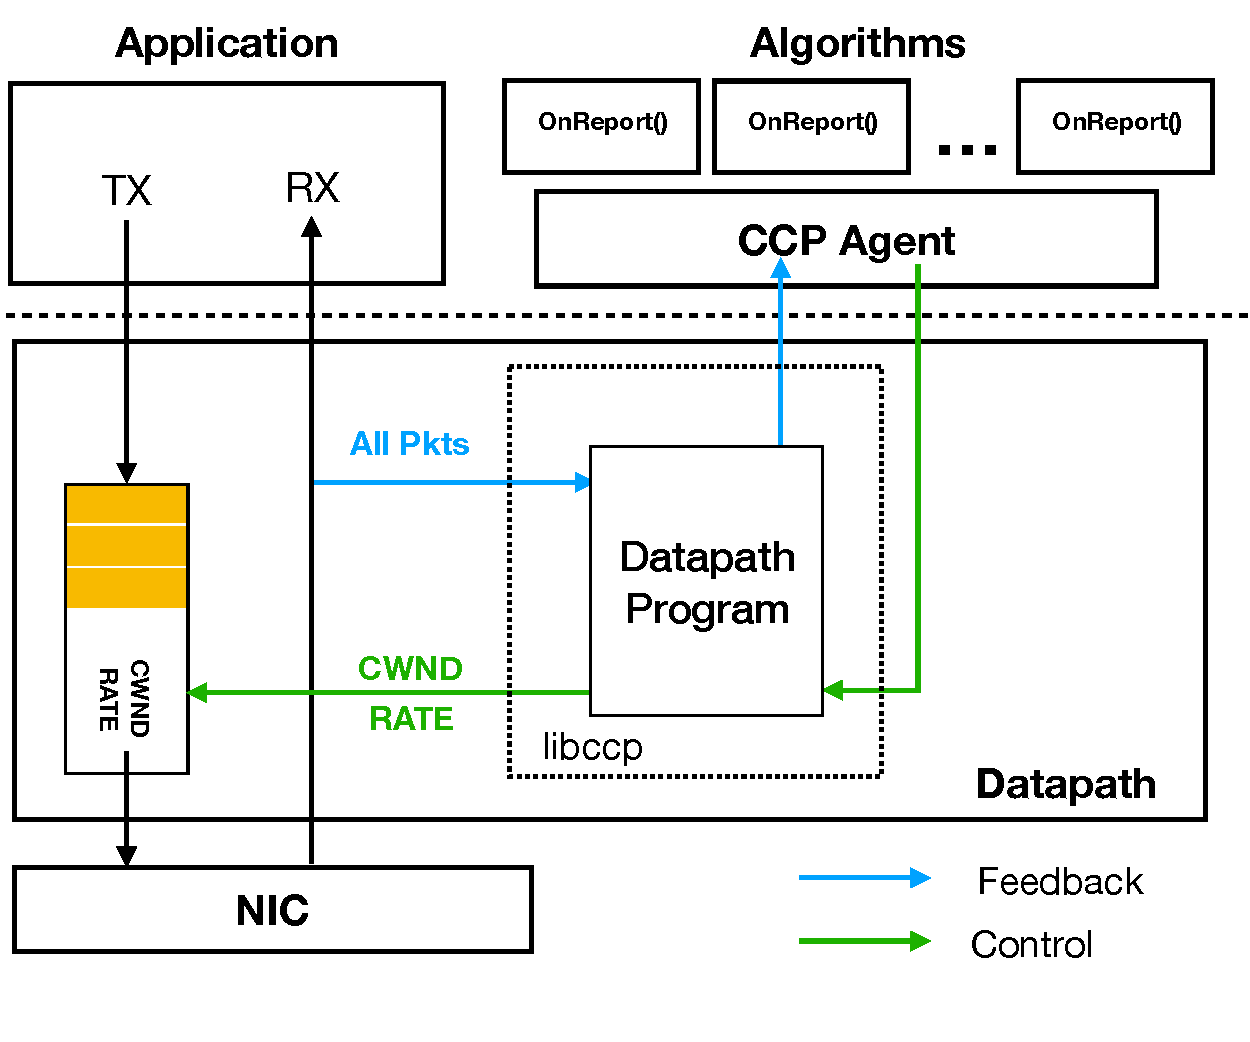
\includegraphics[width=\columnwidth]{img/ccp_design_sigcomm}
    \caption{Congestion control algorithms in CCP are distinct from the application and datapath.
    Users specify control patterns to set the congestion window or rate,
    and fold functions to define how to summarize datapath messages into reports processed in CCP.}\label{fig:design}
\end{figure}
%

To enable rich new congestion control algorithms on datapaths,
CCP must provide a low-barrier programming environment and access
to libraries (\eg for optimization, machine learning, \etc).
%
Further, new algorithms should also achieve high performance running at tens of
Gbit/s per connection with small packet delays in the datapath.

\subsection{Isolating Algorithms from the Datapath}
\label{s:datapath:isolation}
Should congestion control algorithms run in the same address space as the
datapath? There are conflicting factors to consider:

\Para{Safety.} Supporting experimentation with algorithms and the possibility of
including \userspace code means that programs implementing congestion
control algorithms should be considered untrusted. If algorithms and the
datapath are in the same address space, bugs in algorithm or library code could
cause datapath crashes or create vulnerabilities leading to privilege
escalations in the kernel datapath.

\Para{Flexibility.} Placing congestion control functionality outside the datapath provides more flexibility. For example, we anticipate future use cases of the CCP architecture where
a congestion control algorithm may run on a machine different from the sender,
enabling control policies across groups of hosts.

\Para{Performance.} On the other hand, congestion control algorithms can access the datapath's
congestion measurements with low delays and high throughput if the two reside in
the same address space.

Our design restructures congestion control algorithms into two components in
separate address spaces: an off-datapath {\em CCP agent} and a component that
executes in the datapath itself.
%
The CCP agent provides a flexible execution environment in user space for congestion control algorithms, by receiving congestion signals from the datapath
and invoking the algorithm code on these signals.
%
Algorithm developers have full access to the \userspace programming environment, including tools and libraries.
%
The datapath component is responsible for processing feedback (\eg TCP or QUIC
ACKs, packet delays, \etc) from the network and the receiver, and providing congestion signals to the algorithms.
%
Further, the datapath component provides interfaces for algorithms to set
congestion windows and pacing rates.

An alternative design would be to run both the algorithm and the datapath in the same address space, but with fault isolation techniques~\cite{sfi, xfi, bgi, lxfi, nacl, janus, systrace}. 
However, this approach comes with significantly increased CPU utilization (\eg 2$\times$ ~\cite{lxfi, sfi, bgi, janus, systrace}, resulting from tracing and run-time checks), a restrictive development environment~\cite{nacl}, or changes to development tools such as the compiler~\cite{xfi, sfi}.
These performance and usability impediments, in our view, significantly diminish the benefits of running congestion control algorithms and the datapath in one address space.

%% Explicit CCP and datapath separation also enables future use cases where
%% congestion control algorithms may run on a machine different from the sender to
%% centralize congestion control policies across groups of hosts.

%% rephrase the stuff below

\begin{table}[]
    \centering
    \begin{tabular}{c|c|c}
        Implementation & Reporting Interval & Mean Throughput \\
        \hline
        Kernel & - & $43$ Gbit/s \\
        CCP & Per ACK & $29$ Gbit/s \\
        CCP & Per $10$ ms & $41$ Gbit/s \\
    \end{tabular}
    \caption{Single-flow throughput for different reporting intervals between
      the Linux kernel and CCP \userspace, compared to kernel TCP
      throughput. Per-ACK feedback (0 $\mu$s interval) reduces throughput by
      32\% while using a 10 ms reporting interval
      achieves almost identical throughput to the kernel. Results as the number
      of flows  increases are in
      \S\ref{sec:eval:whyfold}.}\label{tab:perf:interval}
      \vspace{-10pt}
\end{table}

\subsection{Decoupling Congestion Control from the ACK Clock}
\label{sec:design:decoupling-cc-from-ack-clock}

Typical congestion control implementations in the Linux kernel are coupled to the so-called ``ACK-clock,'' \ie algorithm functionality is invoked upon receiving a packet acknowledgment in the networking stack.
In contrast, with CCP, algorithms operate on summaries of network observations obtained over multiple measurements gathered in the datapath.
Users program the datapath to gather these summaries using a safe domain-specific language (\S\ref{sec:design:exercising-control-over-datapath}).

This decoupling of algorithm logic from the ACK clock provides two benefits.

First, users can develop congestion control algorithms free from the strict
time restrictions rooted in the inter-arrival time of packet acknowledgments---a useful feature, especially at high link rates.
Hence, it is possible to build algorithms that perform complex computations and yet achieve high throughput.

Second, the ability to provide congestion feedback less frequently than per-ACK can significantly reduce the overhead of datapath-CCP communication.
Table~\ref{tab:perf:interval} shows that for a single saturating \ct{iperf}
connection over a loopback interface, Linux kernel TCP on a server machine
with four 2.8-Ghz cores achieves $45$ Gbit/s running Reno.
In comparison, per-ACK reporting from the kernel to the CCP agent achieves
only 68\% of the kernel's throughput.
By increasing the time between reports sent to the slow path to 10 ms (see the
``per 10 ms'' row), our implementation of Reno in CCP achieves close to the kernel's throughput.

Given that CCP algorithms operate over measurements supplied only infrequently, a key question is how best to summarize congestion signals within the datapath so algorithms can achieve high fidelity compared to a traditional in-datapath implementation.
Indeed, in \S\ref{sec:eval:fidelity} we show that reporting on an RTT time-scale does not affect the fidelity of CCP algorithm implementations relative to traditional in-kernel implementations.

%\subsection{Exercising Control over Datapath Functions}
\subsection{Supporting per-ACK Logic Within the Datapath}
\label{sec:design:exercising-control-over-datapath}
\label{sec:design:restricted-datapath-functions}

How must the datapath provide congestion feedback to algorithms running in the CCP agent?
Ideally, a datapath should supply congestion signals to algorithms with suitable granularity (\eg averaged over an RTT, rather than per ACK), at configurable time intervals (\eg a few times every RTT) and during critical events (\eg packet losses).
With CCP, users can specify such datapath behavior using a domain-specific language (\S\ref{sec:ccp}). 
At a high level, CCP-compatible datapaths expose a number of {\em congestion signals}, over which users can write {\em fold functions} to summarize network observations for algorithms. 
It is also possible to perform \emph{control actions} such as reporting summarized measurements to CCP or setting a flow's pacing rate. 
Datapath programs can trigger fold functions and control actions when certain conditions hold, \eg an ACK is received or a timer elapses.
Users can thus control how to partition the logic of the algorithm between these two components according to their performance and flexibility requirements (\S\ref{s:ccp:ss}).

Figure~\ref{fig:design} shows the architecture of a CCP-enabled sender, highlighting how the components we have discussed in this section fit together. 